\section{Frame}

Let $(Q_t, S_t)$ be a HMM with the amino acid alphabet $\set{A}$.
We want to replace it with a HMM that generates sequences of symbols from the alphabet
$\mathcal B = \{\mathrm A, \mathrm C, \mathrm G, \mathrm T\}$ of DNA bases and is able to account
for frame-shifting.
Let $\mathrm M_j$ be the so-called match state of an amino acid HMM and let $Q_t=\mathrm M_j$.
From the amino acid emission probabilities and any other relevant source of information
(codon usage bias, for instance), one can define the probability $\cprob{X_1=x_1, X_2=x_2, X_3=x_3}{Q_t=\mathrm M_j}$
of $\mathrm M_j$ emitting the codon $(x_1, x_2, x_3) \in \mathcal B^3$
--- one can also write $\cprob{X=x_1x_2x_3}{Q_t=\mathrm M_j}$, for short.
Since measurement errors occur and nature is not perfect, we will replace the
codon emission process by one that instead produces base sequences of different
lengths to account for base insertions and deletions (indels).

Node $\mathrm M_j$ in Fig.~\ref{fig:codon-hmm-tree} represents the modified match state.
The generated codon will go through four transitions, each one representing one of three possibilities: (i) delete a base; (ii) insert a base; or (iii) do nothing.
The deletion can happen in any of the three codon positions with equal probability.
If a deletion has already happened, the next deletion can happen in any of the remaining two positions with equal probability.
The insertion can happen between any two bases, before the first base or after the last base with equal probability.

The codon emitted at node $\mathrm M_j$ can go under $m\in\{0, 1, 2, 3, 4\}$ base indels during
the state transitions that end at some leaf-node state.
The probability of it undergoing $m$ indels is given by
\begin{align*}
    p(M=m) = \binom{4}{4-m} (1 - \eps)^{4-m} \eps^m,
\end{align*}
where coefficient $\binom{4}{m}$ counts the number of paths corresponding to $m$ base indels.
Fig.~\ref{fig:indel-dist} shows the base indel distributions over different values of $\eps$.
Let $F$ be a random variable representing the final sequence length generated by the model in
Fig.~\ref{fig:codon-hmm-tree}.
We have the probabilities
\begin{align*}
    p(F=1) = p(F=5) &= \eps^2(1-\eps)^2, \\
    p(F=2) = p(F=4) &= 2\eps^3(1-\eps) + 2\eps(1-\eps)^3,~\text{and} \\
    p(F=3)          &= \eps^4 + 4\eps^2(1-\eps)^2 + (1-\eps)^4
\end{align*}
illustrated in Fig.~\ref{fig:len-dist} over different values of $\eps$.

\begin{figure}[htbp]
\centering
\begin{subfigure}{.5\textwidth}
  \centering
  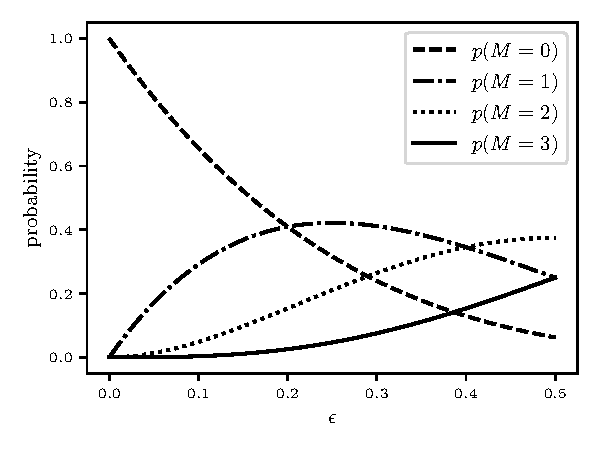
\includegraphics[width=.7\linewidth]{figure/indel-prob}
  \caption{Base indel distribution.}%
  \label{fig:indel-dist}
\end{subfigure}%
\begin{subfigure}{.5\textwidth}
  \centering
  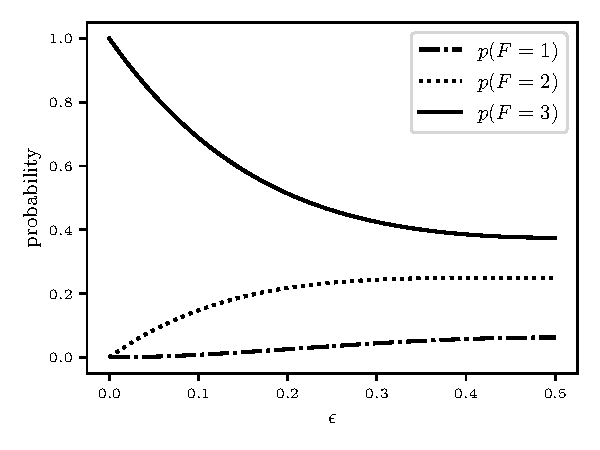
\includegraphics[width=.7\linewidth]{figure/seq-len-prob}
  \caption{Sequence length distribution.}%
  \label{fig:len-dist}
\end{subfigure}
\caption{
    Distribution of base indels and sequence length over the transition probability $\eps$.
    It is recommended to choose a value for $\eps$ that is smaller than $1/5$ such that
    $p(M=m)<p(M=m+1)$, as per Fig.~\ref{fig:indel-dist}.
}
\label{fig:dist}
\end{figure}

A sequence $\mathbf z=z_1 z_2\dots$ of finite but variable length will emerge at the end of the
process represented in Fig.~\ref{fig:codon-hmm-tree}.
Let $\mathcal Q_f$ be the set of hidden paths, starting with $Q_t=\mathrm M_j$ and ending at some leaf-node state,
that generate sequences of length $f$.
Let $Z^f=(Z^f_1, \dots, Z^f_f)$ be a $f$-tuple of random variables that generates such sequences of length $f$.
We have
\begin{align*}
    p(Z^f=z_1\dots z_f,F=f) &= \sum_{\mathbf q \in \mathcal Q_f}
    \cprob{Z^f=z_1\dots z_f}{Q_{t..t+4}=\mathbf q} p(Q_{t..t+4}=\mathbf q).
\end{align*}
